\subsection{Gewindesteigung \hfill ME}
\begin{footnotesize}
    \begin{itemize}
        \item $P$ = Gewindesteigung = Zurückgelegter Weg bei einer Umdrehung
        \item Bsp.: M30 x 2 $\to$ $d = 30, P = 2$ (P angegeben $\rightarrow$ Feingewinde)
    \end{itemize}
    \begin{minipage}{0.58\linewidth}
        \begin{center}
            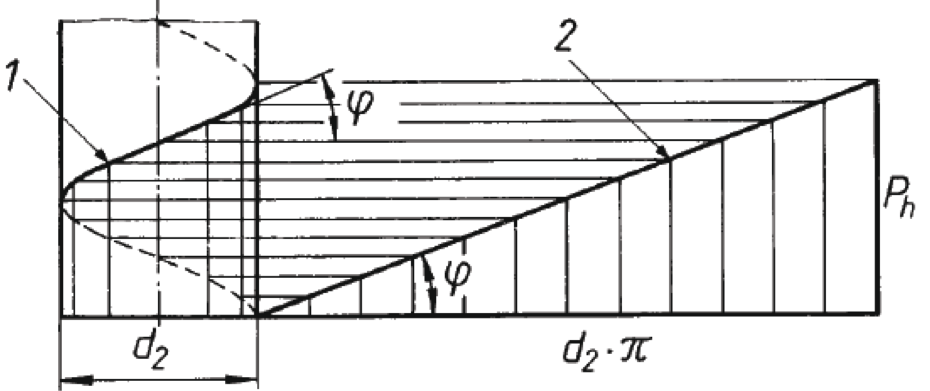
\includegraphics[width = 0.8\linewidth]{MAEIP_Gewindesteigung}
            \mathbox{
                tan(\varphi) = \frac{P}{2\pi \cdot r_m} = \frac{P}{\pi \cdot d_2}
            }
        \end{center}
    \end{minipage}
    \begin{minipage}{0.4\linewidth}
        \begin{center}
            \begin{align*}
                \varphi &= \text{Steigungswinkel}
                \\ P &= \text{Gewindesteigung}
                \\ d_2 &= \text{Flankendurchmesser}
            \end{align*}
            \mathbox{
                \# \text{Umdrehungen} = \frac{\text{Distanz}}{P}
            }
        \end{center}
    \end{minipage}
    \begin{empheq}[box=\fbox]{align*}
        &\text{Regelsteigung (wenn bei Deklaration keine Angabe steht): }\\
        &P = 1.75 mm \text{Abhängig von Schraubendurchmesser}
    \end{empheq}
\end{footnotesize}